%
% Chapter Introduction
%
\chapter{Developer Manual}
This chapter holds detailed information for software developers who want to modify or extend DICOMUX. The code is currently under heavy development and the class diagram is only valid for the date of creation.\\
A JavaDoc page including a class diagram is available and can be downloaded from dicomux.org.

\section{Terminology}
\paragraph{Plug-in}
This term is used for classes which extend the abstract class APlugin. These classes are designated to extend DICOMUX in order to support the visualization of one or more Dicom elements.
\paragraph{Dicom element}
A variable or attribute of the type org.dcm4che2.data.DicomElement.
\paragraph{Dicom object}
A variable or attribute of the type org.dcm4che2.data.DicomObject.
\paragraph{Workspace}
This term refers to a selectable tab in the View. All workspaces are independant from each other. A workspace is represented by a TabObject which holds all related information.

\section{Architecture}
The architecture of DICOMUX is based on the model-view-controller pattern. Furthermore, the application can be extended by adding plug-ins. The user always interacts either with the View or with several plug-ins.

\subsection{MVC}
This design helps to improve the modularization of the application. Each component of this pattern got its own interface. This doesn't serve a certain purpose yet.

\subsubsection{Model}
The class Model implements IModel and is designated to hold the entire state of the application. This includes all open Dicom files, all workspaces with their selected plug-ins and so on.
\paragraph{TabObject} is a class which serves as data transfer object between Model and View. It represents a workspace and holds all necessary information for visualization.
\paragraph{TabState} is an enum which is part of each TabObject. It represents the state a workspace can have.

\subsubsection{View}
The class View implements IView and holds the user interface without having any complex algorithms. The view uses the model as source of information and manages the available languages. The View gets informated by the Model when new data is available. In that case, the View reloads everything. Furthermore, the View informs the Controller if the user did a state changing input like opening a Dicom file, changing the selected plug-in, exiting the application and so on. Opening the file menu is not a state changing input and will not be reported to the Controller.

\subsubsection{Controller}
The class Controller implements IController and serves as manager between View and Model. The View informs the Controller if the user did a serious input. The Controller will take all necessary actions in order to handle the request. If the user requests a Dicom file to be opened, the Controller will create a new workspace. That workspace will be filled with the selected Dicom file, a suitable plug-in and some more information. After that, the Controller will add the new workspace to the Model.

\subsection{Plug-in mechanism}
Each plug-in has to extend the abstract class APlugin. After implementing all necessary methods, the new plug-in has to be added to the Controller's constructor. This mechanism is not innovative but functional. Each plug-in has to add Dicom Tags to its m\_keyTag attribute in order to enable a Controller to determine for which Dicom Tags this plug-in can be used for.\\
User interaction has to be handled by the plug-ins themselves. They have to provide a user interface and all necessary algorithms. 
\paragraph{KeyTag} is a class which which supports the Controller in his automatic plug-in selection procedures. Each plug-in has an attribute of the type KeyTag which holds all necessary information for this purpose.

\section{Graphical User Interface}
As described in the user guide, the user interface of DICOMUX is based on workspaces. There are no pop-up windows which confuse and disturb the user.

\subsection{States}
The user interface including its workspaces can have different states. The following state diagram visualizes this.

		\begin{minipage}{\textwidth} 
		\centering
		\fbox{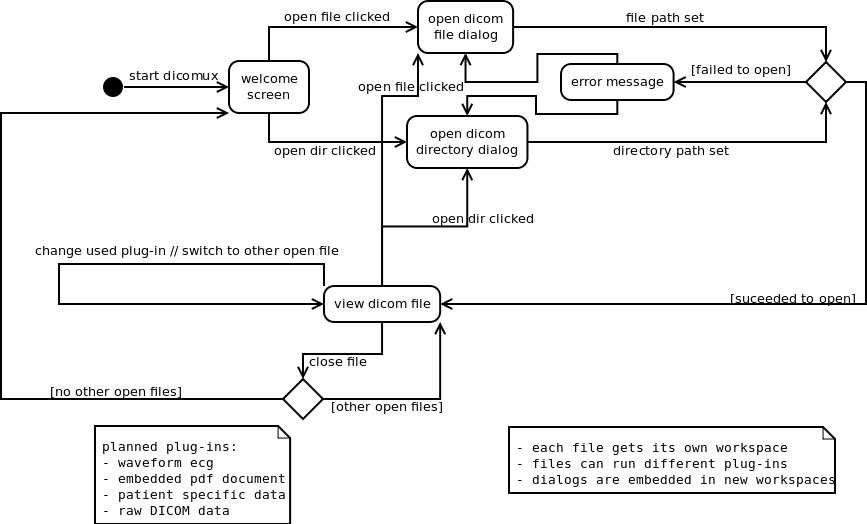
\includegraphics[width=\linewidth]{screens/stateDiagram.png}}
		\captionof{figure}{States of the user interface}
		\label{fig:bild}
		\end{minipage}

%
% EOF
%